\documentclass{article}

% Formatting
\usepackage[utf8]{inputenc}
\usepackage[margin=1in]{geometry}
\usepackage[titletoc,title]{appendix}
\usepackage{listings}
\usepackage{float}

% Math
\usepackage{amsmath,amsfonts,amssymb,mathtools}
\usepackage[ruled,vlined]{algorithm2e}
\usepackage{algorithmic}


% Images
\usepackage{graphicx}
\graphicspath{ {./images/} }

% Tables
\usepackage{booktabs}

% References
\usepackage{biblatex}
\addbibresource{references.bib}

% Title content
\title{CS 434 HW4}
\author{Tristan Gavin}
\date{May 20, 2021}

\begin{document}

\maketitle

\section*{Written Exercises: Analyzing Naive Bayes}
\subsection*{Q1. Prove Bernoulli Naive Bayes has a linear decision boundary}
\begin{align*}
    &\frac{P(y=1|x_1,...,x_d)}{P(y=0|x_1,...,x_d)} > 1 \\[1em] 
    &\implies log(1) < log(P(y=1|x_1,...,x_d))-log(P(y=0|x_1,...,x_d)) \\[1em]
    &\implies 0 < log[\theta_1\prod_{i=1}^d\theta_{i1}^{xi}(1-\theta_{i1})^{1-x_i}]-log[\theta_0\prod_{i=1}^d\theta_{i0}^{xi}(1-\theta_{i0})^{1-x_i}] \\[1em]
    & = log(\theta_1)+\sum_{i=1}^d[x_ilog(\theta_1)+(1-x_i)log(1-\theta_{i1})] - log(\theta_0)-\sum_{i=1}^d[x_ilog(\theta_0)+(1-x_i)log(1-\theta_{i0})] \\[1em]
    & = log(\theta_1) - log(\theta_0) + \sum_{i=1}^dx_ilog(\theta_1) - \sum_{i=1}^dx_ilog(\theta_0) + \sum_{i=1}^d(1-x_i)log(1-\theta_{i1}) - \sum_{i=1}^d(1-x_i)log(1-\theta_{i0}) \\[1em]
    & = log(\frac{\theta_1}{\theta_0})+\sum_{i=1}^dx_ilog\frac{\theta_1}{\theta_0}+\sum_{i=1}^d(1-x_i)log(\frac{1-\theta_{i1}}{1-\theta_{i0}}) \\[1em]
    &= log(\frac{\theta_1}{\theta_0})+\sum_{i=1}^dx_ilog\frac{\theta_1}{\theta_0} + \sum_{i=1}^dlog(\frac{1-\theta_{i1}}{1-\theta_{i0}})  - \sum_{i=1}^dx_ilog(\frac{1-\theta_{i1}}{1-\theta_{i0}}) \\[1em]
    &= log(\frac{\theta_1}{\theta_0}) + \sum_{i=1}^dx_i[log\frac{\theta_1}{\theta_0}- log\frac{1-\theta_{i1}}{1-\theta_{i0}}] + \sum_{i=1}^dlog(\frac{1-\theta_{i1}}{1-\theta_{i0}})  \\[1em]
    &\implies log(\frac{\theta_1}{\theta_0}) + \sum_{i=1}^dlog(\frac{1-\theta_{i1}}{1-\theta_{i0}}) + \sum_{i=1}^dx_i[log\frac{\theta_1}{\theta_0}- log\frac{1-\theta_{i1}}{1-\theta_{i0}}] > 0  \\
\end{align*}
This is in form $b+ \sum_{i=1}^dw_ix_i > 0$ where \[b = log(\frac{\theta_1}{\theta_0}) + \sum_{i=1}^dlog(\frac{1-\theta_{i1}}{1-\theta_{i0}}), \quad \quad w_i = log\frac{\theta_1}{\theta_0}- log\frac{1-\theta_{i1}}{1-\theta_{i0}}\]

\subsection*{Q2. Duplicate Features in Naïve Bayes}
    TODO

\section*{Implementing a Neural Network For Digit Identification}
\subsection*{Q3. Implementing the Backward Pass for a Linear Layer}
There wasn't anything that needed to be reported for this question but I will post the plot that is given using the default hyperparamaters for reference for later questions.

\begin{figure}[H]
    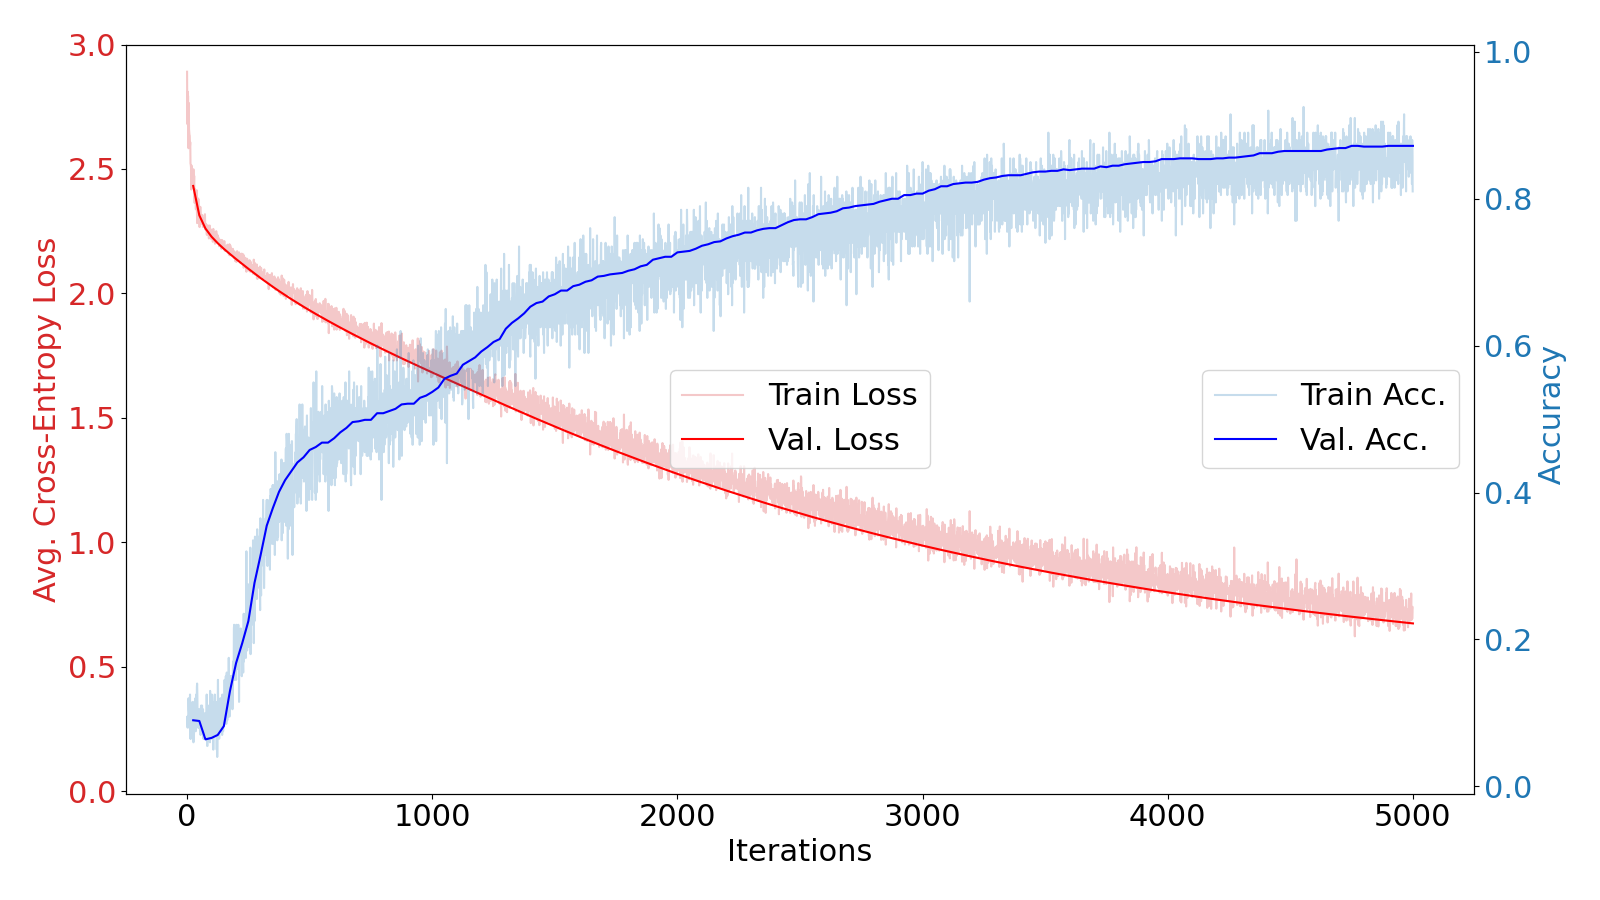
\includegraphics[scale = 0.4]{default.png} 
\end{figure}

\section*{Analyze Hyperparamaters}
\subsection*{Q4. Adjusting Learning Rates}
\begin{figure}[H]
    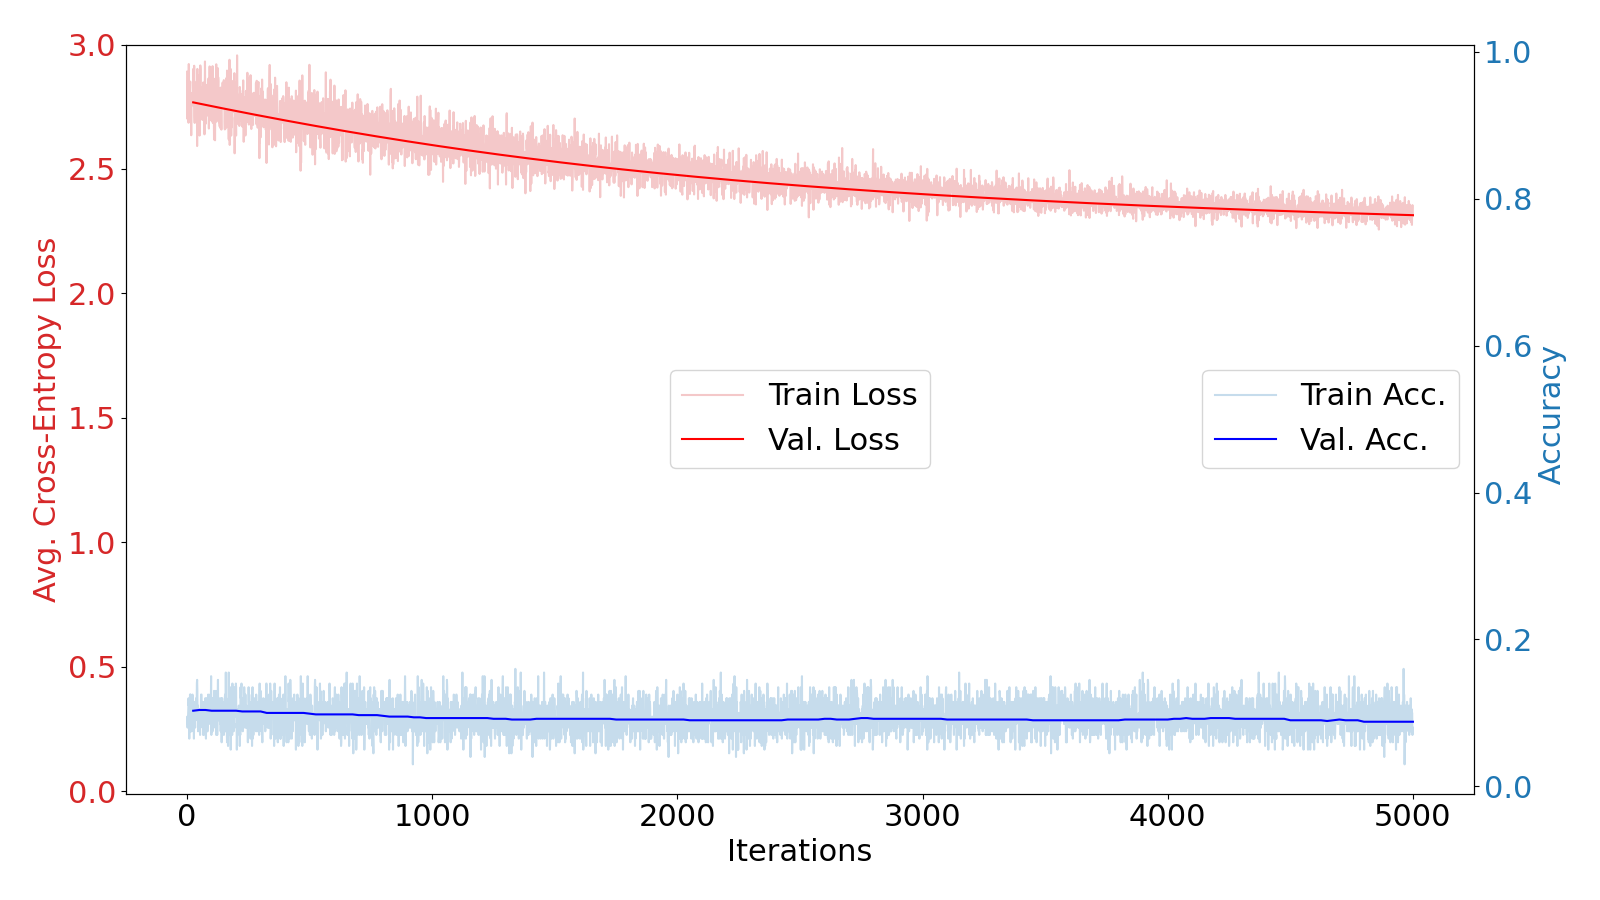
\includegraphics[scale = 0.4]{step.0001.png} 
    \caption{step size of 0.0001 (everything else default)}
\end{figure}
\begin{figure}[H]
    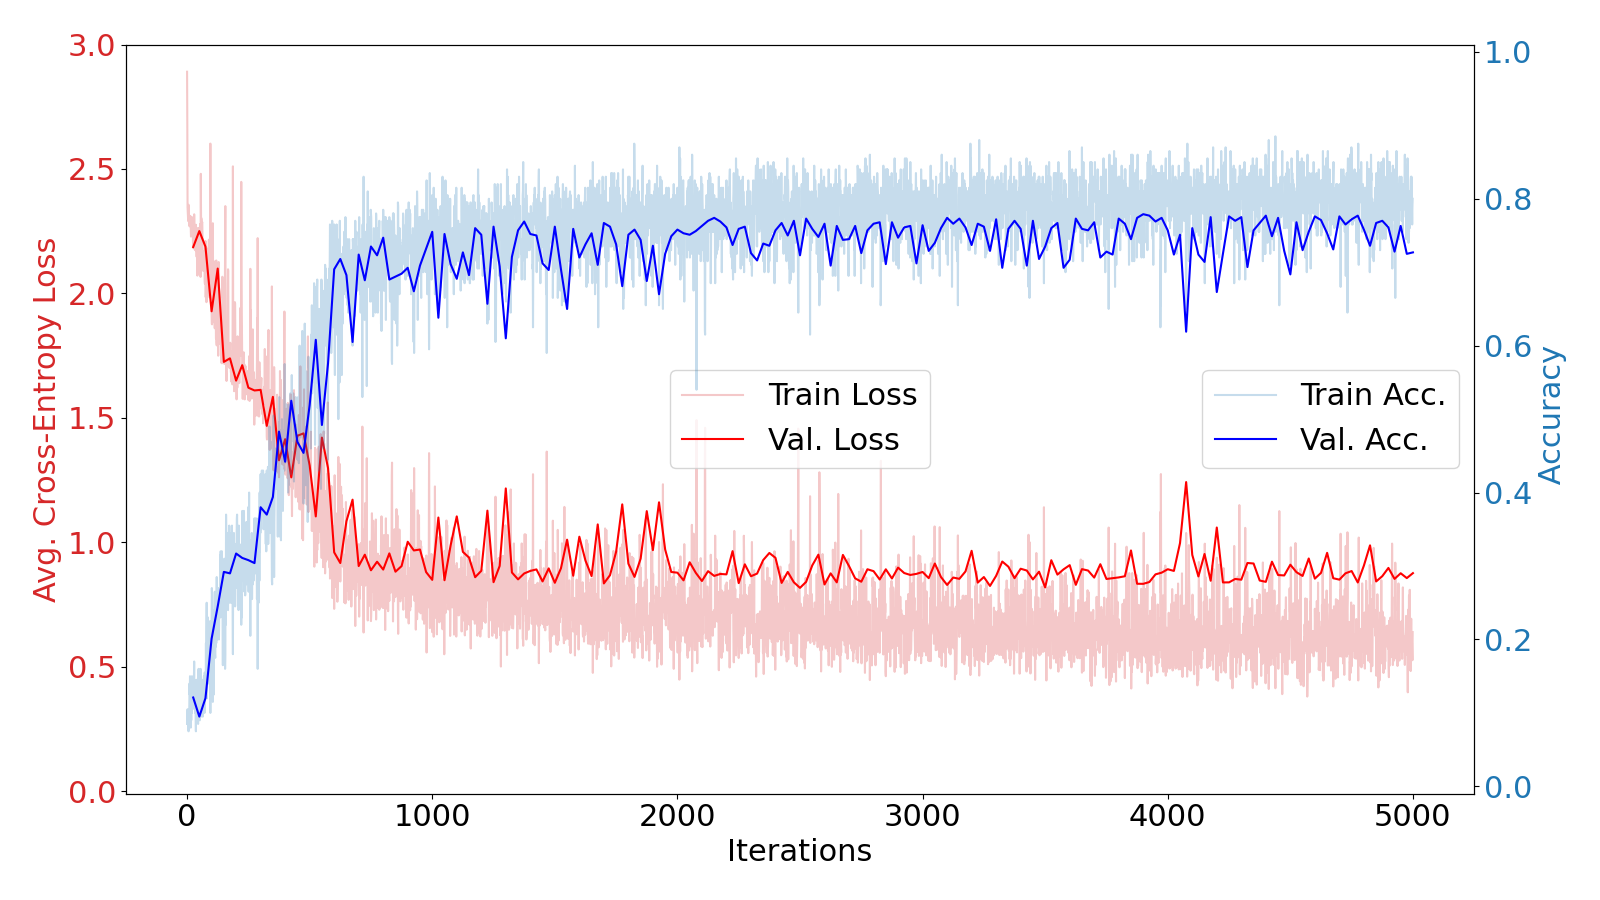
\includegraphics[scale = 0.4]{step5.png} 
    \caption{step size of 5 (everything else default)}
\end{figure}
\begin{figure}[H]
    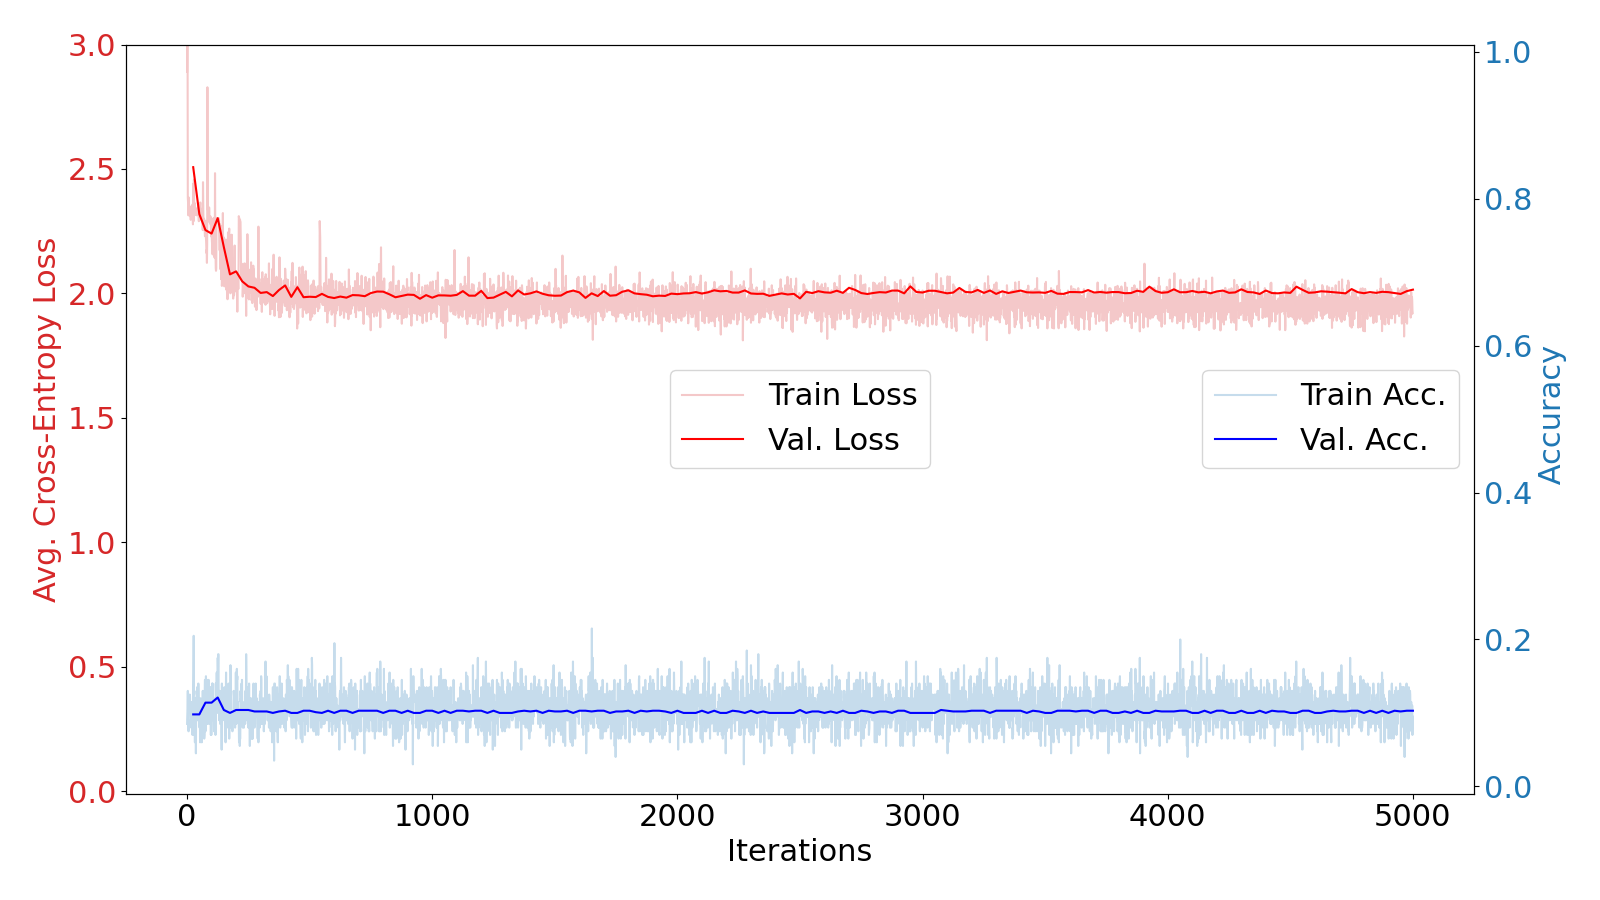
\includegraphics[scale = 0.4]{step10.png} 
    \caption{step size of 10 (everything else default)}
\end{figure}

\subsubsection*{Compare and contrast}

Step size 0.0001: \\[1em]
(a) The final training accuracy was 9.26\% and the validation accuracy ended at 8.8\%. This step size was too small to see any improvement over just 200 iterations. What was suprising to me was that although the average Cross-entropy loss got smaller after more epochs, the accuracy on both validation and test actually got worse. Somehow we were getting less loss but a higher error rate. \\[1em]
(b) After seeing the validation accuracy decrease as iterations increased, I expected that trend to continue if we increased the epochs, but when I actually cranked the max epochs up to 1000 the validation and training accruacy did slowly start to improve. After 1000 epochs they had improved to 22\% and were still slowly increasing. \\[1em]
Step size 5: \\[1em]
(a)Training Accuracy - 79.98\%, Validation Accuracy - 72.7\%. We see in the graph a lot of variance with this step size on each epoch. This is probably because the step size over shoots the local minimum and ends up going to worse weights some times. However the step size is good enough to converge to something at least close to a local optimum. It's accuracy is much worse than the default hyperparameters.\\[1em]
(b) My initial guess for what will happen as max epochs is increased is that the average training and validation accuracy will stay about the same and continue to oscilate as the weights bounce around the local minimum. When testing this hypothesis with 1000 epochs this was mostly the case but there was a peculiar large jump in accruacy at epoch 360, where the training accuracy went from about 80\% to 90\% in one itteration. My guess is that maybe the function was randomly able to get unstuck from a local optimum and find a better maybe more global optimum.\\[1em]
\pagebreak

\noindent Step size 10: \\[1em]
(a)Training Accuracy - 10.18\%, Validation Accuracy - 10.3\%. This step size fails to converge to a local optimum. The step size is far too big so every step it takes overshoots an optimal weight setting. I would have expected the error to be more variant but it actually stays pretty smooth. This might be because the algorithm is so bad that it is essentially guessing randomly and therefore always has a 10\% chance of getting the right answer.\\[1em]
(b) I do not think that increasing the max epochs will have any effect. The step size is so large that we wil never be able converge to any kind of minimum. (after testing on a max epoch of 1000 my hypothesis was confirmed.)

\subsubsection*{ReLU's and Vanishing Gradients}
\begin{figure}[H]
    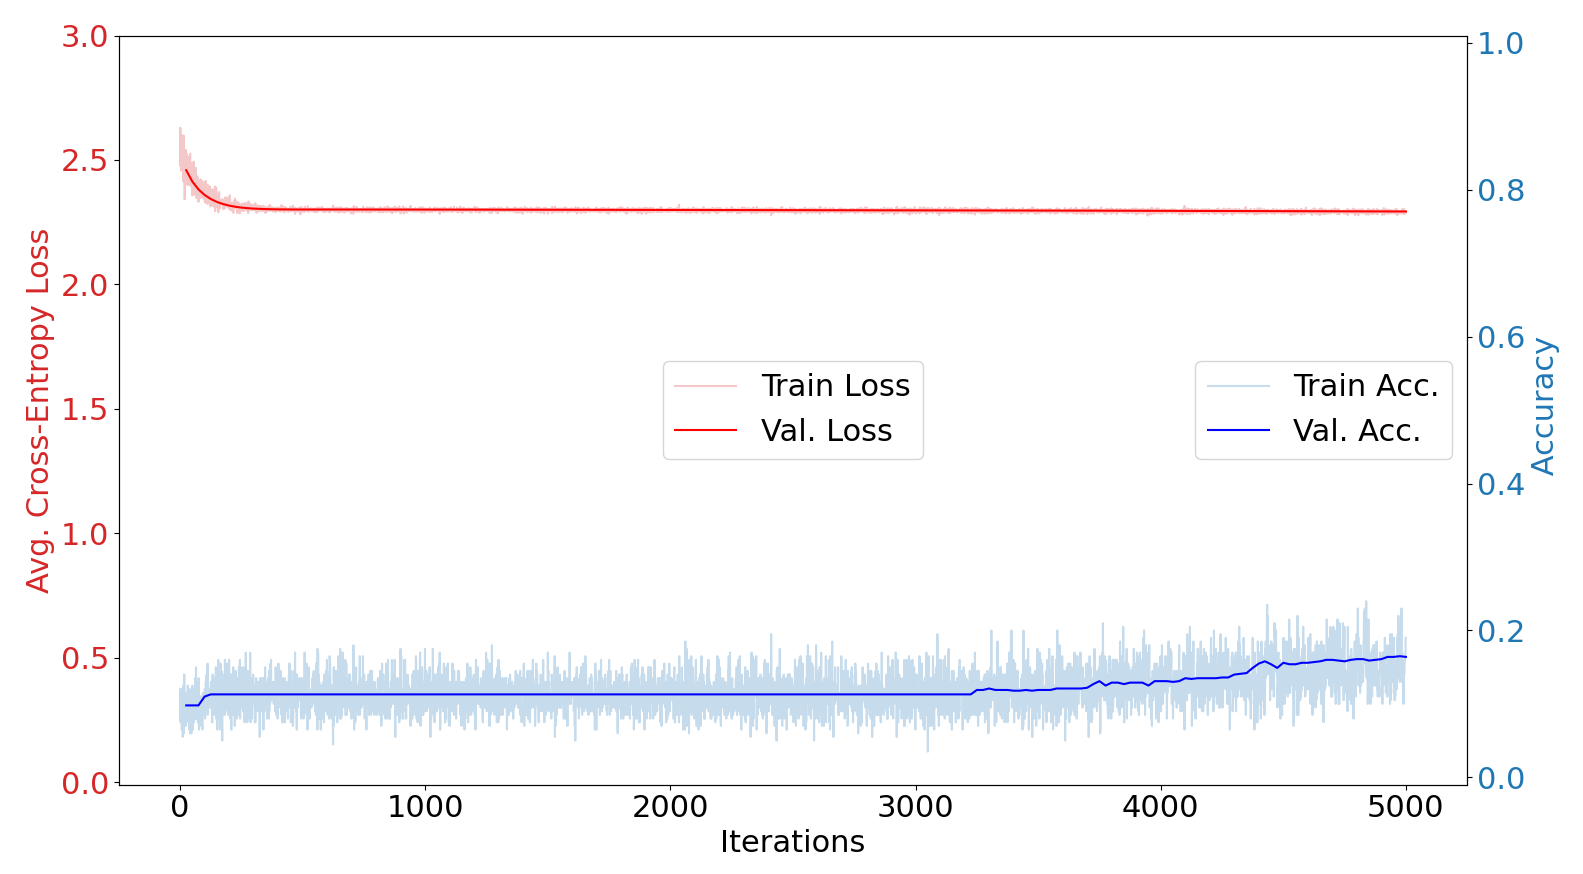
\includegraphics[scale = 0.4]{5layersigmoid.png} 
    \caption{5-layer with Sigmoid Activation (default values for other hyperparameters)}
\end{figure}
\begin{figure}[H]
    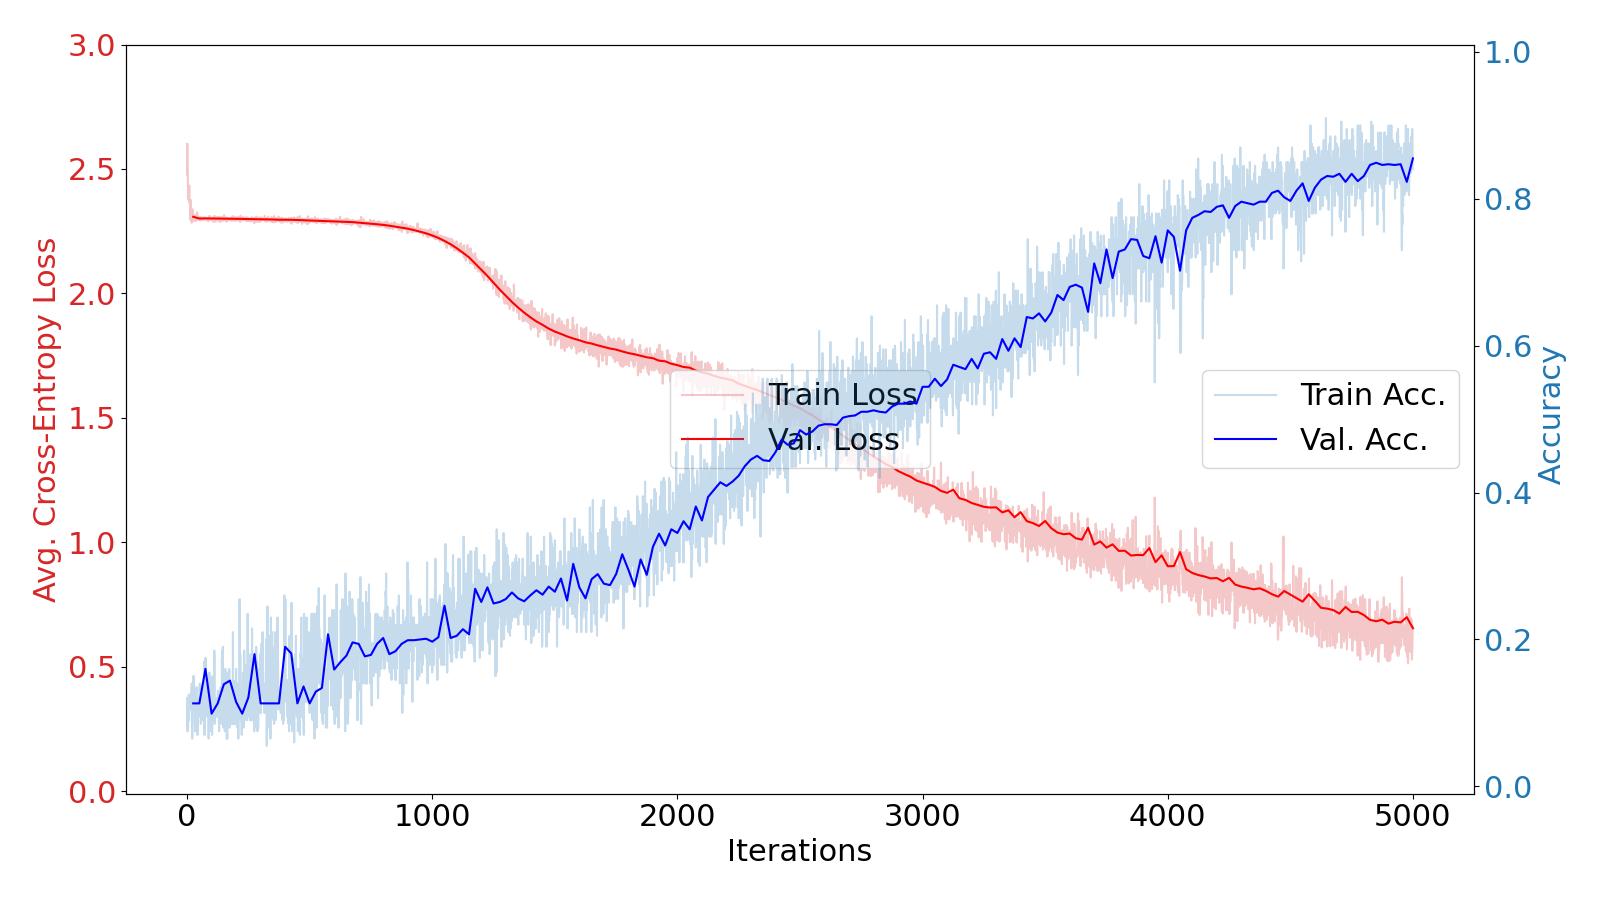
\includegraphics[scale = 0.4]{layers5step.1.png} 
    \caption{5-layer with Sigmoid Activation with 0.1 step size (default values for other hyperparameters)}
\end{figure}
\begin{figure}[H]
    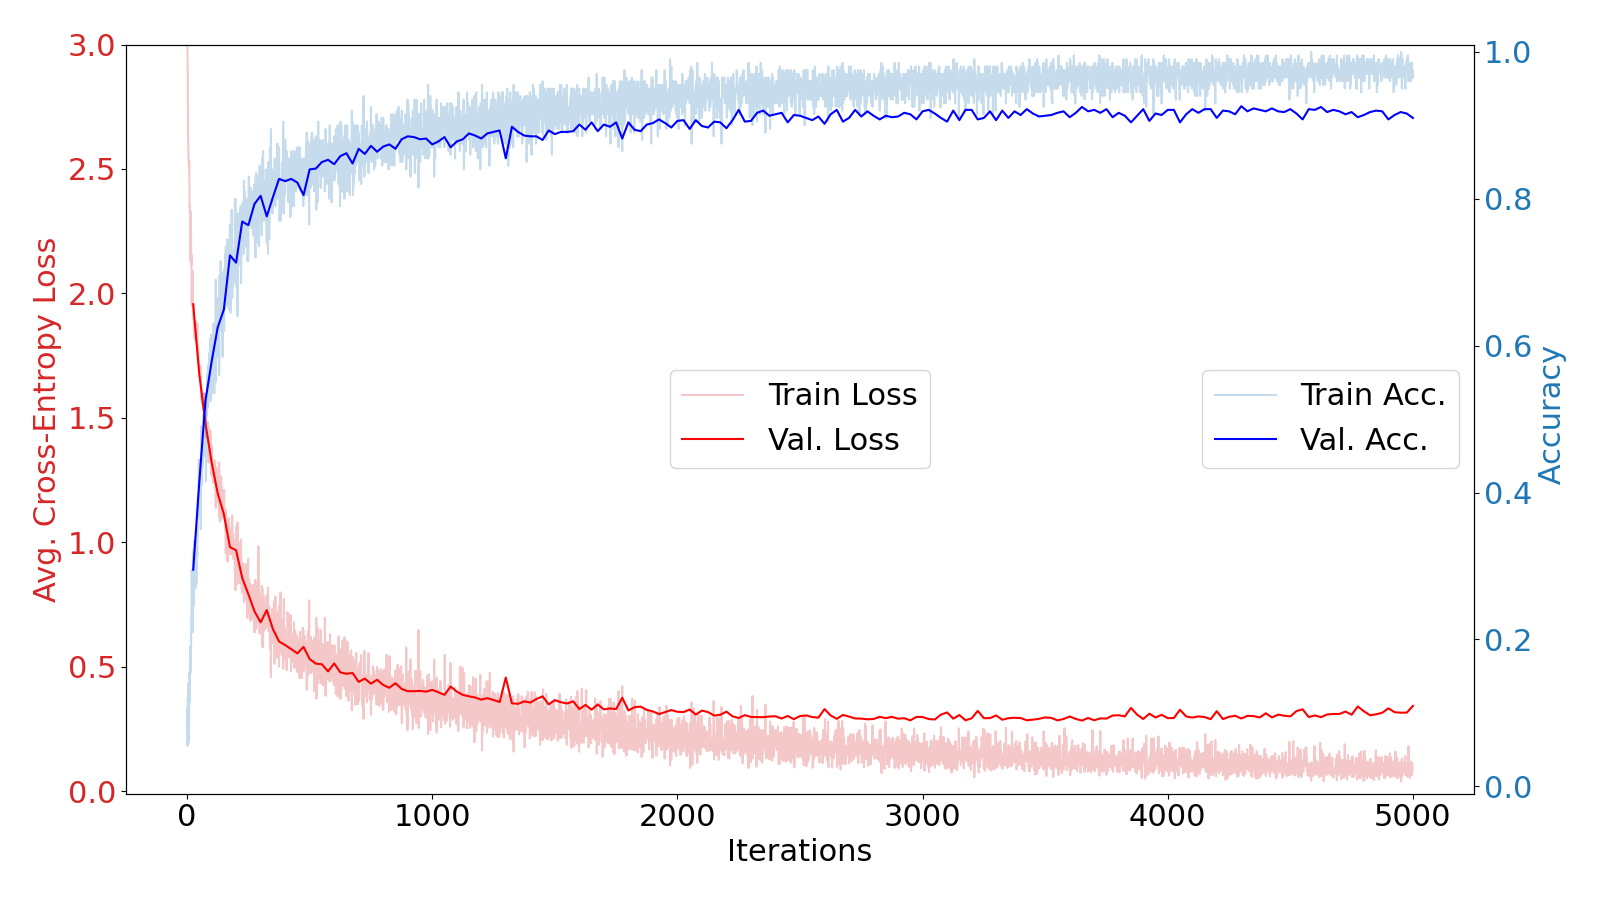
\includegraphics[scale = 0.4]{layers5relu.png} 
    \caption{5-layer with ReLU Activation (default values for other hyperparameters)}
\end{figure}

5-layer with Sigmoid Activation:\\[1em]
(a) Similar to the default hyperparamaters there is a quick ininitial decrease in the loss, but here that drecrease levels out very quickly and remains flat for the rest of the iterations about about 2.3. Training and test accruacy slowly increase throughout the itterations but after reaching the max epoch of 200 they only reach about 15.6\% for train and 16.4\% for test. Increasing the number of layers actually made our programs accuracy worse in this case.\\[1em]
5-layer with Sigmoid Activation with 0.1 step size: \\[1em]
(a) Increasing the step size by a magnitude of 10 helped a lot in the 5-layer sigmoid activation neural net. After max epoch of 200 the accuracy reached 86\% for train and 85\% for validation. This is almost the same accuracy that we got on the default hyperparameters with just two layers, however the 5 layer accuracy oscilates significantly more (more jagged graph). The other difference I noticed is that in the 2-layer sigmoid has a much quicker increase in accuracy at the very begining and then starts to flatten out quickly where as the 5-layer sigmoid activation is more gradual or linear as it increases in accuracy. It makes more of an X shape with the loss curve. \\[1em]



\end{document}
